\documentclass[14pt]{beamer}

% Assets
\usepackage[czech]{babel}				% Jazyk
\usepackage[a-2u]{pdfx}					% Kopírování z pdfka
\usepackage{tikz}						% Schémata automatů
\usepackage{csquotes}					% české uvozovky
\usepackage{enumerate}					% enumerate environment
\usepackage{indentfirst}
\usepackage{mathtools}
\usepackage{pifont}
\usepackage{xcolor}
\usepackage{enumitem,xcolor}
\usepackage{amsmath}
\usepackage[utf8]{inputenc}

\usepackage{listings}                   % Úryvky z kódu (C#)
\lstset{language=[Sharp]C, frame=lr}
% Beamer theme
\usetheme{Boadilla}
\setbeamertemplate{frame numbering}[fraction]
\usecolortheme[named=black]{structure}
\setbeamertemplate{navigation symbols}{}
\setbeamerfont{title}{series=\bfseries,parent=structure}
\setbeamerfont{frametitle}{series=\bfseries,parent=structure}
\usefonttheme[onlymath]{serif}
\urlstyle{same}

% Dark theme
\setbeamercolor{frametitle}{fg=white}
\setbeamercolor{title}{fg=white}
\setbeamercolor{background canvas}{bg=black}
\setbeamercolor{normal text}{fg=white}

\defbeamertemplate*{title page}{customized}[1][]
{ 
  \usebeamerfont*{title}\inserttitle\par
  \bigskip
  \usebeamerfont*{subtitle}\textit{\insertsubtitle}\par
  \bigskip \bigskip \bigskip \bigskip 
  \usebeamerfont{author}\insertauthor\par
  \usebeamerfont{institute}Kabinet \office\\\url{weber3@spsejecna.cz}\bigskip
}
% Enumerate
%\setlist[enumerate]{topsep=0pt,itemsep=-1ex,partopsep=1ex,parsep=1ex,label=(\arabic*)}

\MakeOuterQuote{"}

% Colors
\definecolor{lightblue}{HTML}{009AD4}
\definecolor{darkgreen}{HTML}{0D7103}
\definecolor{lightgreen}{HTML}{68FF00}
\definecolor{darkred}{HTML}{AF0B0B}
\definecolor{lightred}{HTML}{FF5100}
\definecolor{orange}{HTML}{FFE000}
\definecolor{codeblue}{HTML}{FF0055}
\definecolor{codegreen}{rgb}{0,0.6,0}
\definecolor{codegray}{rgb}{0.5,0.5,0.5}
\definecolor{codebeige}{HTML}{D4A000}
\definecolor{backcolour}{rgb}{0.95,0.95,0.92}

\newcommand{\markred}[1]{\textcolor{lightred}{#1}}
\newcommand{\markgreen}[1]{\textcolor{lightgreen}{#1}}
\newcommand{\markorange}[1]{\textcolor{orange}{#1}}
\newcommand{\markblue}[1]{\textcolor{lightblue}{#1}}

% Inline images
\newcommand{\inlineimgscale}{1.1}

% X and check mark
\newcommand{\cmark}{\markgreen{\ding{51}}}
\newcommand{\xmark}{\markred{\ding{55}}}

% Redefinions
\renewcommand{\implies}{\Rightarrow}
\renewcommand{\impliedby}{\Leftarrow}

% Math
\newcommand{\R}{\mathbb{R}}
\newcommand{\C}{\mathbb{C}}
\newcommand{\N}{\mathbb{N}}
\newcommand{\Z}{\mathbb{Z}}
\newcommand{\Q}{\mathbb{Q}}

% Code
\lstdefinestyle{clang}{
    basicstyle=\small\ttfamily\color{white},
    language=C,
    keywordstyle=\color{codeblue},
    commentstyle=\color{codegreen},
    numberstyle=\tiny\color{codegray},
    stringstyle=\color{codebeige},
    breakatwhitespace=false,
    breaklines=true,
    captionpos=b,
    keepspaces=true,
    numbersep=5pt,
    showspaces=false,
    showstringspaces=false,
    showtabs=false,
    morekeywords={void,int,double,float,unsigned,if,else,\#include}
    tabsize=0.5
}
\lstset{escapeinside={(*}{*)},style=clang}

\newcommand{\hlcode}[1]{\colorbox{red}{#1}}

% Title page
\title{Informační a komunikační technologie}
\subtitle{První pohled na jazyk C}
\author{David Weber}
\def\office{K13}
\def\email{weber3@spsejecna.cz}

\begin{document}

    % Itemize
    \setlist[itemize]{label=\textcolor{white}{\textbullet}}

    % Verbatims
    \defverbatim{\basicconstruction}{\begin{verbatim}
        
    \end{verbatim}}


    % Slides
    \begin{frame}
        \titlepage
    \end{frame}

    \begin{frame}[t]{Co už jsme probrali}
        \begin{itemize}
            \item Zápis programu pomocí
            \begin{itemize}
                \item \markorange{plošného strukturogramu} a
                \item \markorange{vývojového diagramu}.
            \end{itemize}
            \item Typy příkazů
            \begin{itemize}
                \item \markorange{jednoduchá činnost (např. přiřazení do proměnné)},
                \item \markorange{podmínka (větvení programu)},
                \item \markorange{iterace s testem na začátku/konci}.

            \end{itemize}
            \item Krokování programu
        \end{itemize}
        \begin{center}
            \markgreen{$\implies$ Máme určitou představu, jak programy fungují} \emoji{slightly-smiling-face}
        \end{center}
    \end{frame}

    \begin{frame}[t]{S čím budeme pracovat?}
        \begin{itemize}
            \item Jazyků existuje celá řada
            \begin{itemize}
                \item \only<1>{C}\only<2>{$\boxed{\text{C}}$}, C++, C\#, Java, Python, Rust, \dots
            \end{itemize}
            \item Různé odlišnosti:
            \begin{itemize}
                \item technická implementace,
                \item syntaxe,
                \item způsob programovaní (tzv. programovací paradigma),
                \item \dots
            \end{itemize}
        \end{itemize}
    \end{frame}

    \begin{frame}[t]{Stručně k jazyku C}
        \begin{columns}[t]
            \begin{column}{.75\textwidth}
                \begin{itemize}
                    \item Vyvinut v 70. letech
                    \item Nízkoúrovňový programovací jazyk
                    \item \markorange{Kompilovaný (překládaný)} přímo do strojového kódu
                    \item Trvale se používá při programování
                    \begin{itemize}
                        \item operačních systémů,
                        \item ovladačů zařízení,
                        \item jednočipových počítačů,
                        \item \dots
                    \end{itemize}
                \end{itemize}
            \end{column}
            \begin{column}{.25\textwidth}
                \begin{figure}[H]
                    \centering
                    
\includegraphics[scale=.25]{images/C_programming_language_logo.pdf}
                \end{figure}
            \end{column}
        \end{columns}
    \end{frame}

    \begin{frame}[t]{V čem budeme pracovat?}
        \begin{itemize}
            \item K psaní kódu bychom nám technicky stačil poznámkový blok
            \begin{center}
                \markred{$\implies$ to by bylo celkem nepraktické!}
            \end{center}
            \item Lepší bude použít tzv. IDE (Integrated Developer Environment)
            \begin{itemize}
                \item Poskytne nám např. \markorange{zvýraznění syntaxe, autocomplete, aj.}
            \end{itemize}
            \item Na cvičeních se setkáte s
            \begin{itemize}
                \item \markorange{\textbf{Visual Studio Code}} \only<2>{\markgreen{$\impliedby$ budeme používat} \emoji{slightly-smiling-face}}
                \item \markorange{\textbf{Code::Blocks}}
                \item \markorange{\textbf{OnlineGDB}} (online kompilátor, \href{https://www.onlinegdb.com/online_c_compiler}{\underline{odkaz}})
            \end{itemize}
        \end{itemize}
    \end{frame}
    
    \begin{frame}[t]{První spuštění VS Code}
        \begin{figure}
            \centering
            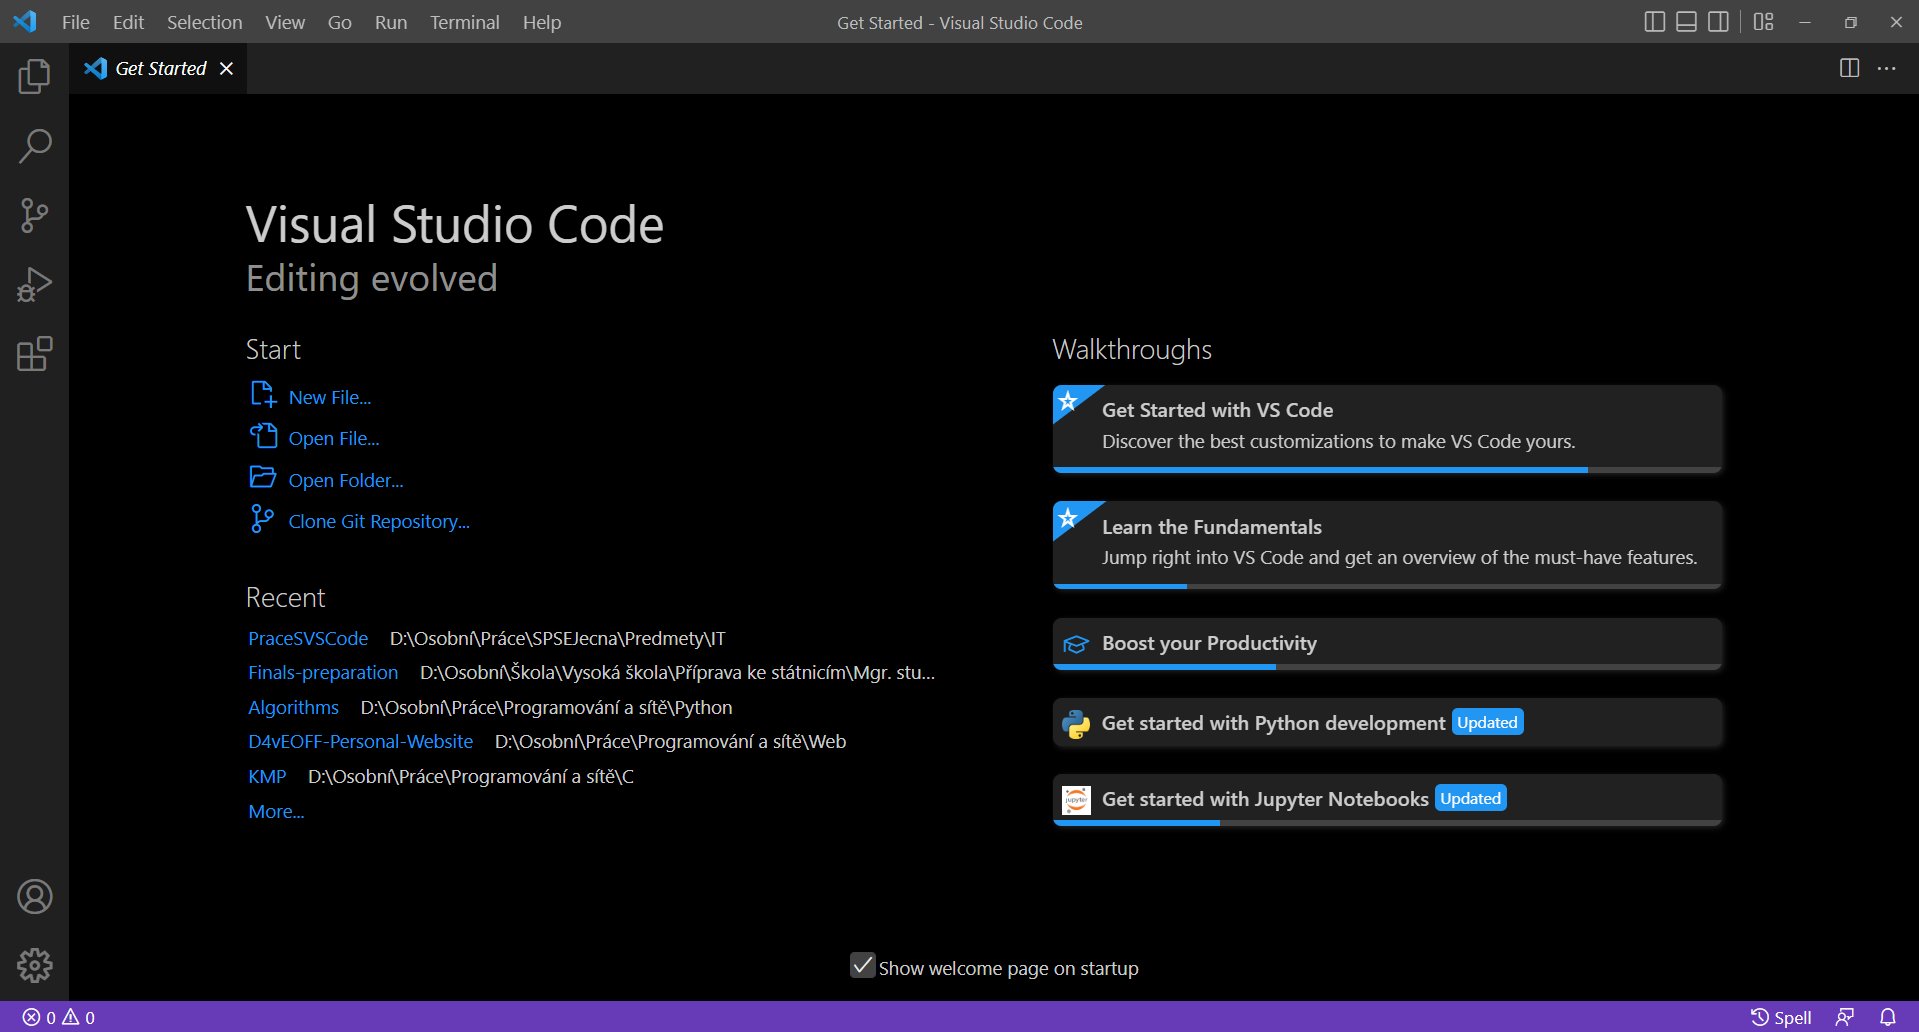
\includegraphics[width=.9\textwidth]{images/vs_code_first_launch.png}
        \end{figure}
    \end{frame}

    \begin{frame}[t]{Prostředí VS Code}
        \begin{itemize}
            \item V levém menu pro nás budou důležité možnosti:
            \begin{itemize}
                \item 
\includegraphics[height=\inlineimgscale\fontcharht\font`\B]{images/vs_code_files_icon.png} \markorange{$\leftarrow$ struktura projektu (složky)}
                \item 
\includegraphics[height=\inlineimgscale\fontcharht\font`\B]{images/vs_code_extensions_icon.png} \markorange{$\leftarrow$ rozšíření pro VS Code}
            \end{itemize}
            \item Později využijeme i tlačítka 
\includegraphics[height=\inlineimgscale\fontcharht\font`\B]{images/vs_code_search_icon.png} a 
\includegraphics[height=\fontcharht\font`\B]{images/vs_code_debug_icon.png}.
            \item Horní menu:
            \begin{itemize}
                \item \markorange{\emph{File $\rightarrow$ Open File}} (otevření souboru)
                \item \markorange{\emph{File $\rightarrow$ Open Folder}} (otevření složky)
            \end{itemize}
        \end{itemize}
    \end{frame}

    \begin{frame}[t]{Rozšíření do VS Code}
        \begin{itemize}
            \item Budeme potřebovat pouze rozšíření \markorange{C/C++} pro autocomplete.
            \item Upravení vzhledu
            \begin{itemize}
                \item \markorange{Black+ Material} $\leftarrow$ tmavé pozadí v editoru
                \item \markorange{Material Icon Theme} $\leftarrow$ hezčí ikonky \emoji{slightly-smiling-face}
            \end{itemize}
        \end{itemize}
    \end{frame}

    \begin{frame}[t]{Kompilátor}
        \begin{itemize}
            \item Čistě s VS Code nám program ještě fungovat nebude. \emoji{worried-face}
        \end{itemize}
        \begin{center}
            \markorange{$\implies$ Kód programu potřebujeme přeložit!}
        \end{center}
        \begin{itemize}
            \item K tomu slouží tzv. \markorange{kompilátor (překladač).}
        \end{itemize}
    \end{frame}

    \begin{frame}[t]{Schéma kompilace}
        \begin{figure}[h]
            \centering
            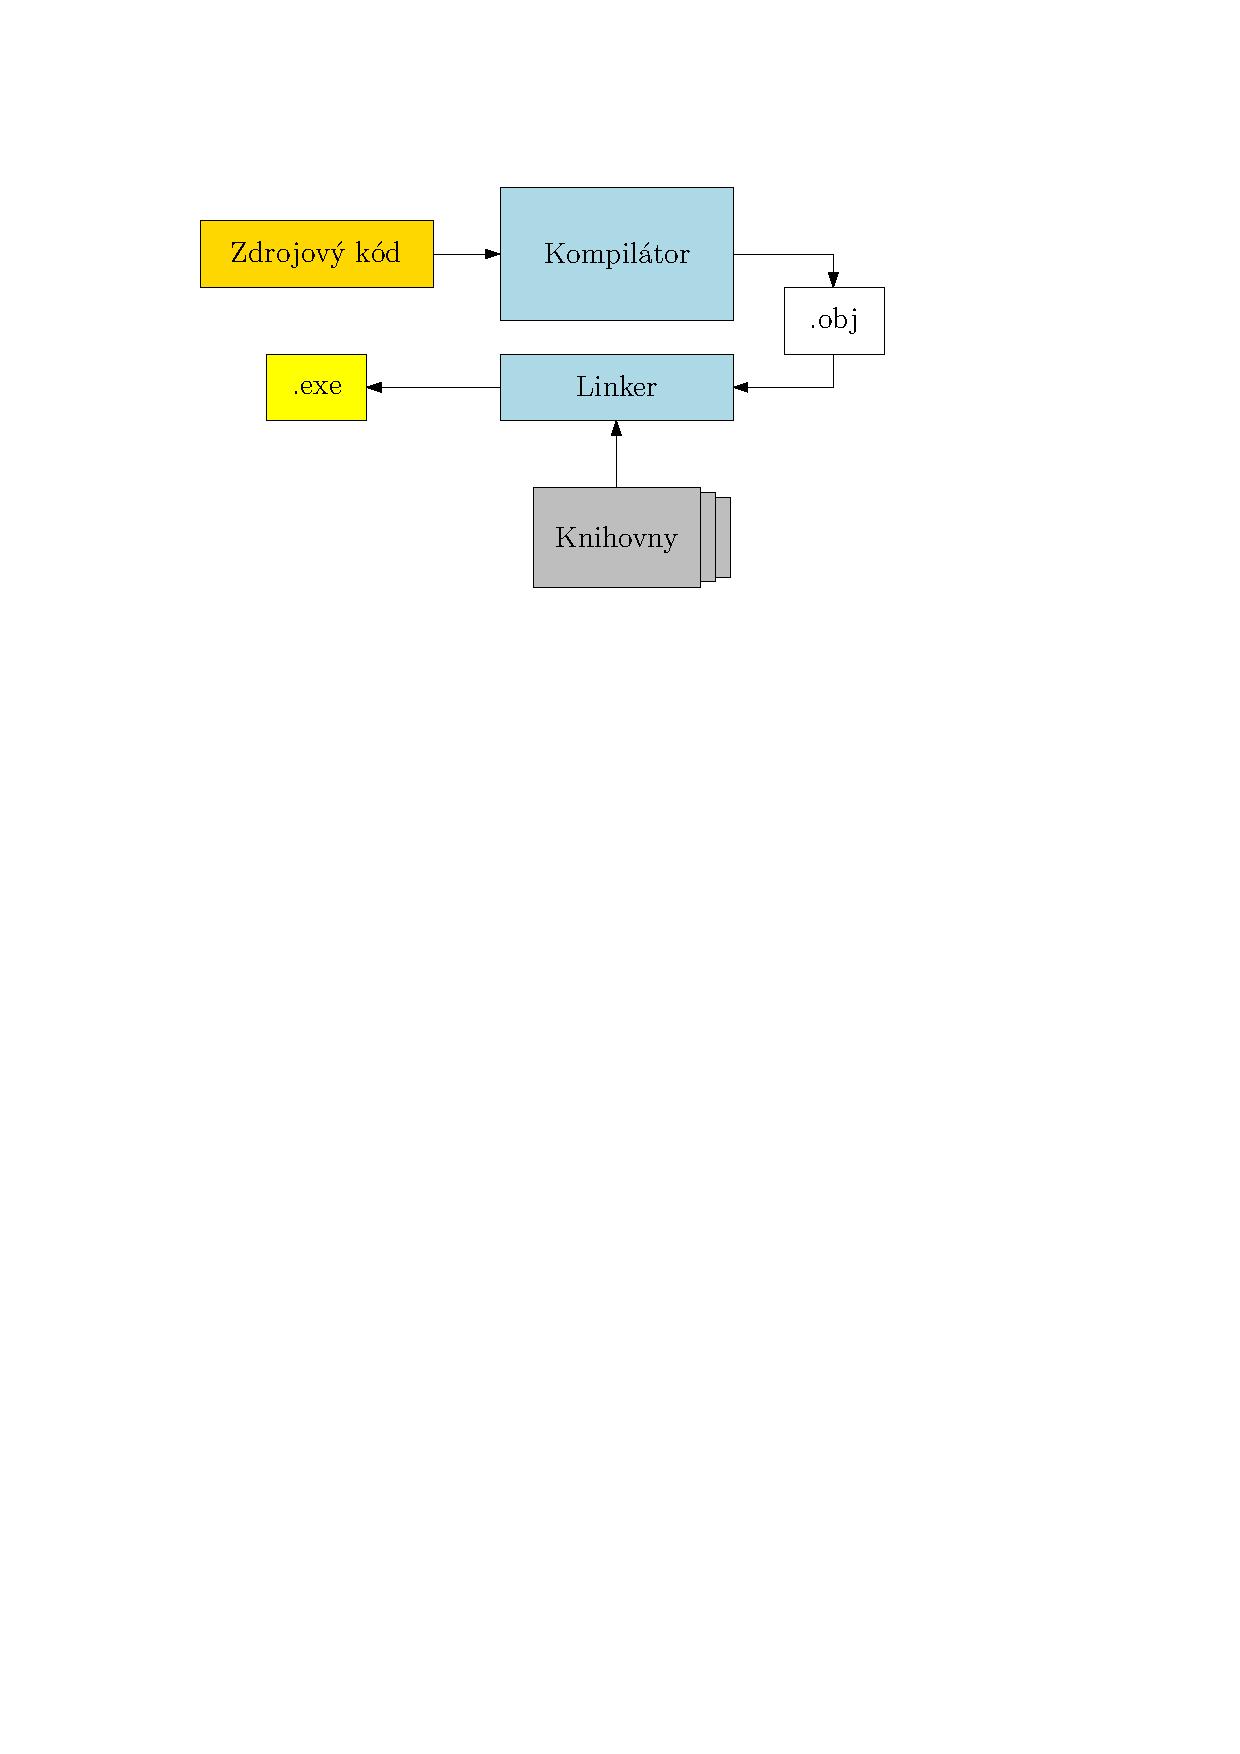
\includegraphics[scale=.8]{images/compiling.pdf}
        \end{figure}
    \end{frame}

    \begin{frame}[t]{Kompilátor}
        \begin{itemize}
            \item Kompilátorů pro jazyk C existuje mnoho
            \begin{itemize}
                \item \markorange{GCC, TCC, Clang, Lattice C, \dots}
            \end{itemize}
            \item Mnohé zároveň podporují i jazyk C++.
            \item Většina linuxových distribucí implicitně obsahuje GCC kompilátor.
            \item Pro MS Windows existují jeho porty
            \begin{itemize}
                \item \markorange{MinGW, Cygwin, \dots}
            \end{itemize}
        \end{itemize}
    \end{frame}

    \begin{frame}[t,fragile]{Základy jazyka C}
        \begin{itemize}
            \item Základní konstrukce programu
            \begin{lstlisting}
int main(void) {
    // Kód programu

    return 0;
}
            \end{lstlisting}
            \item Řádek \texttt{int main(void)} je požadovaný vstup do programu.
            \item Příkazy, které chceme, aby program vykonal, vkládáme mezi složené závorky \{, \}.
            \item Kód v jazyce C ukládáme do souborů s koncovkou \texttt{.c}.
        \end{itemize}
    \end{frame}

    \begin{frame}[t]{Základy jazyka C}
        \begin{itemize}
            \item Představme si, že bychom chtěli, aby program vypsal naše jméno.
            \item K tomu složí příkaz \texttt{printf}.
        \end{itemize}
        \begin{center}
            \markred{$\implies$ To zatím nemůžeme!} \emoji{worried-face}
        \end{center}
        \begin{itemize}
            \item Potřebujeme přidat tzv. \markorange{knihovnu}, která jej definuje.
            \begin{itemize}
                \item Souhrn \markorange{procedur} a \markorange{funkcí}
            \end{itemize}
        \end{itemize}
        \begin{center}
            \markgreen{$\implies$ Klíčové slovo \texttt{\#include}.}
        \end{center}
        \begin{itemize}
            \item Do programu umístíme odkaz na knihovnu \texttt{stdio} (Standard Input/Output)
        \end{itemize}
    \end{frame}

    \begin{frame}[t,fragile]{Základy jazyka C}
        \begin{itemize}
            \item Do kódu programu přidáme knihovnu příkazem
            \begin{center}
                \texttt{\#include <stdio.h>}.
            \end{center}
            Soubory \texttt{.h} značí \markorange{hlavičkové soubory} (zatím nebudeme řešit \emoji{slightly-smiling-face}).
            \begin{lstlisting}
#include <stdio.h>

int main(void) {
    // Kód programu

    return 0;
}
            \end{lstlisting}
        \end{itemize}
    \end{frame}

    \begin{frame}[t,fragile]{Základy jazyka C}
        \begin{itemize}
            \item Posloupnost znaků zapisujeme mezi uvozovky \markorange{\textquotedbl{} \textquotedbl} (neplést s \markorange{' '}).
            \begin{lstlisting}
#include <stdio.h>

int main(void) {
    printf("David Weber");

    return 0;
}
            \end{lstlisting}
        \end{itemize}
    \end{frame}

    \begin{frame}[t]{Základy jazyka C}
        \begin{itemize}
            \item Aby program byl spustitelný, musíme jej nejdříve zkompilovat.
            \item To provedeme v konzoli, kterou ve VS Code otevřeme přes \markorange{\emph{Terminal $\rightarrow$ New Terminal}}, příkazem
            \begin{center}
                \texttt{gcc \textbf{<soubor>} -o \textbf{<výstupní soubor>}}
            \end{center}
            \item U jména výstupního souboru není třeba uvádět typ, tj. \texttt{.exe}; při kompilaci je doplněn automaticky. \emoji{slightly-smiling-face}
        \end{itemize}
    \end{frame}

    \begin{frame}{Otázky?}
        \begin{figure}
            \centering
            
\includegraphics[scale=.4]{images/discussion_inverted.png}
        \end{figure}
    \end{frame}

\end{document}